\documentclass[11pt]{article}
%
\usepackage{basic}
%
\title{Case study: $A_3$}
\begin{document}
\maketitle
%
Let us investigate the case $\nu = (1,2,1) = \alpha_1 + 2\alpha_2 + \alpha_3$ with $\kpf(\nu) = 5$. We are interested in the multidegrees, equivariant multiplicities, and Hilbert series of the five MV cycles $\irr\overline{S^0\cap T^\nu}$ so we begin by describing their ideals.

\begin{question}
    Does there exist some natural order on Lusztig data? aka, on Kostant partitions? 
\end{question}

\noindent Fix the order $3 < 2 < 1$ on $I$ and the reduced expression $\uvi = (1,2,3,1,2,1)$ for $w_0\in W$. 

\begin{description}
    \item[{\bf 1.} $n_\bullet = (0,1,0,1,0,1)$:] $\lambda = (4,3,1,0)$ and $\mu = (3,2,2,1)$ 
    \hfill
 
    % \begin{figure}[ht!]
    % \begin{center}
        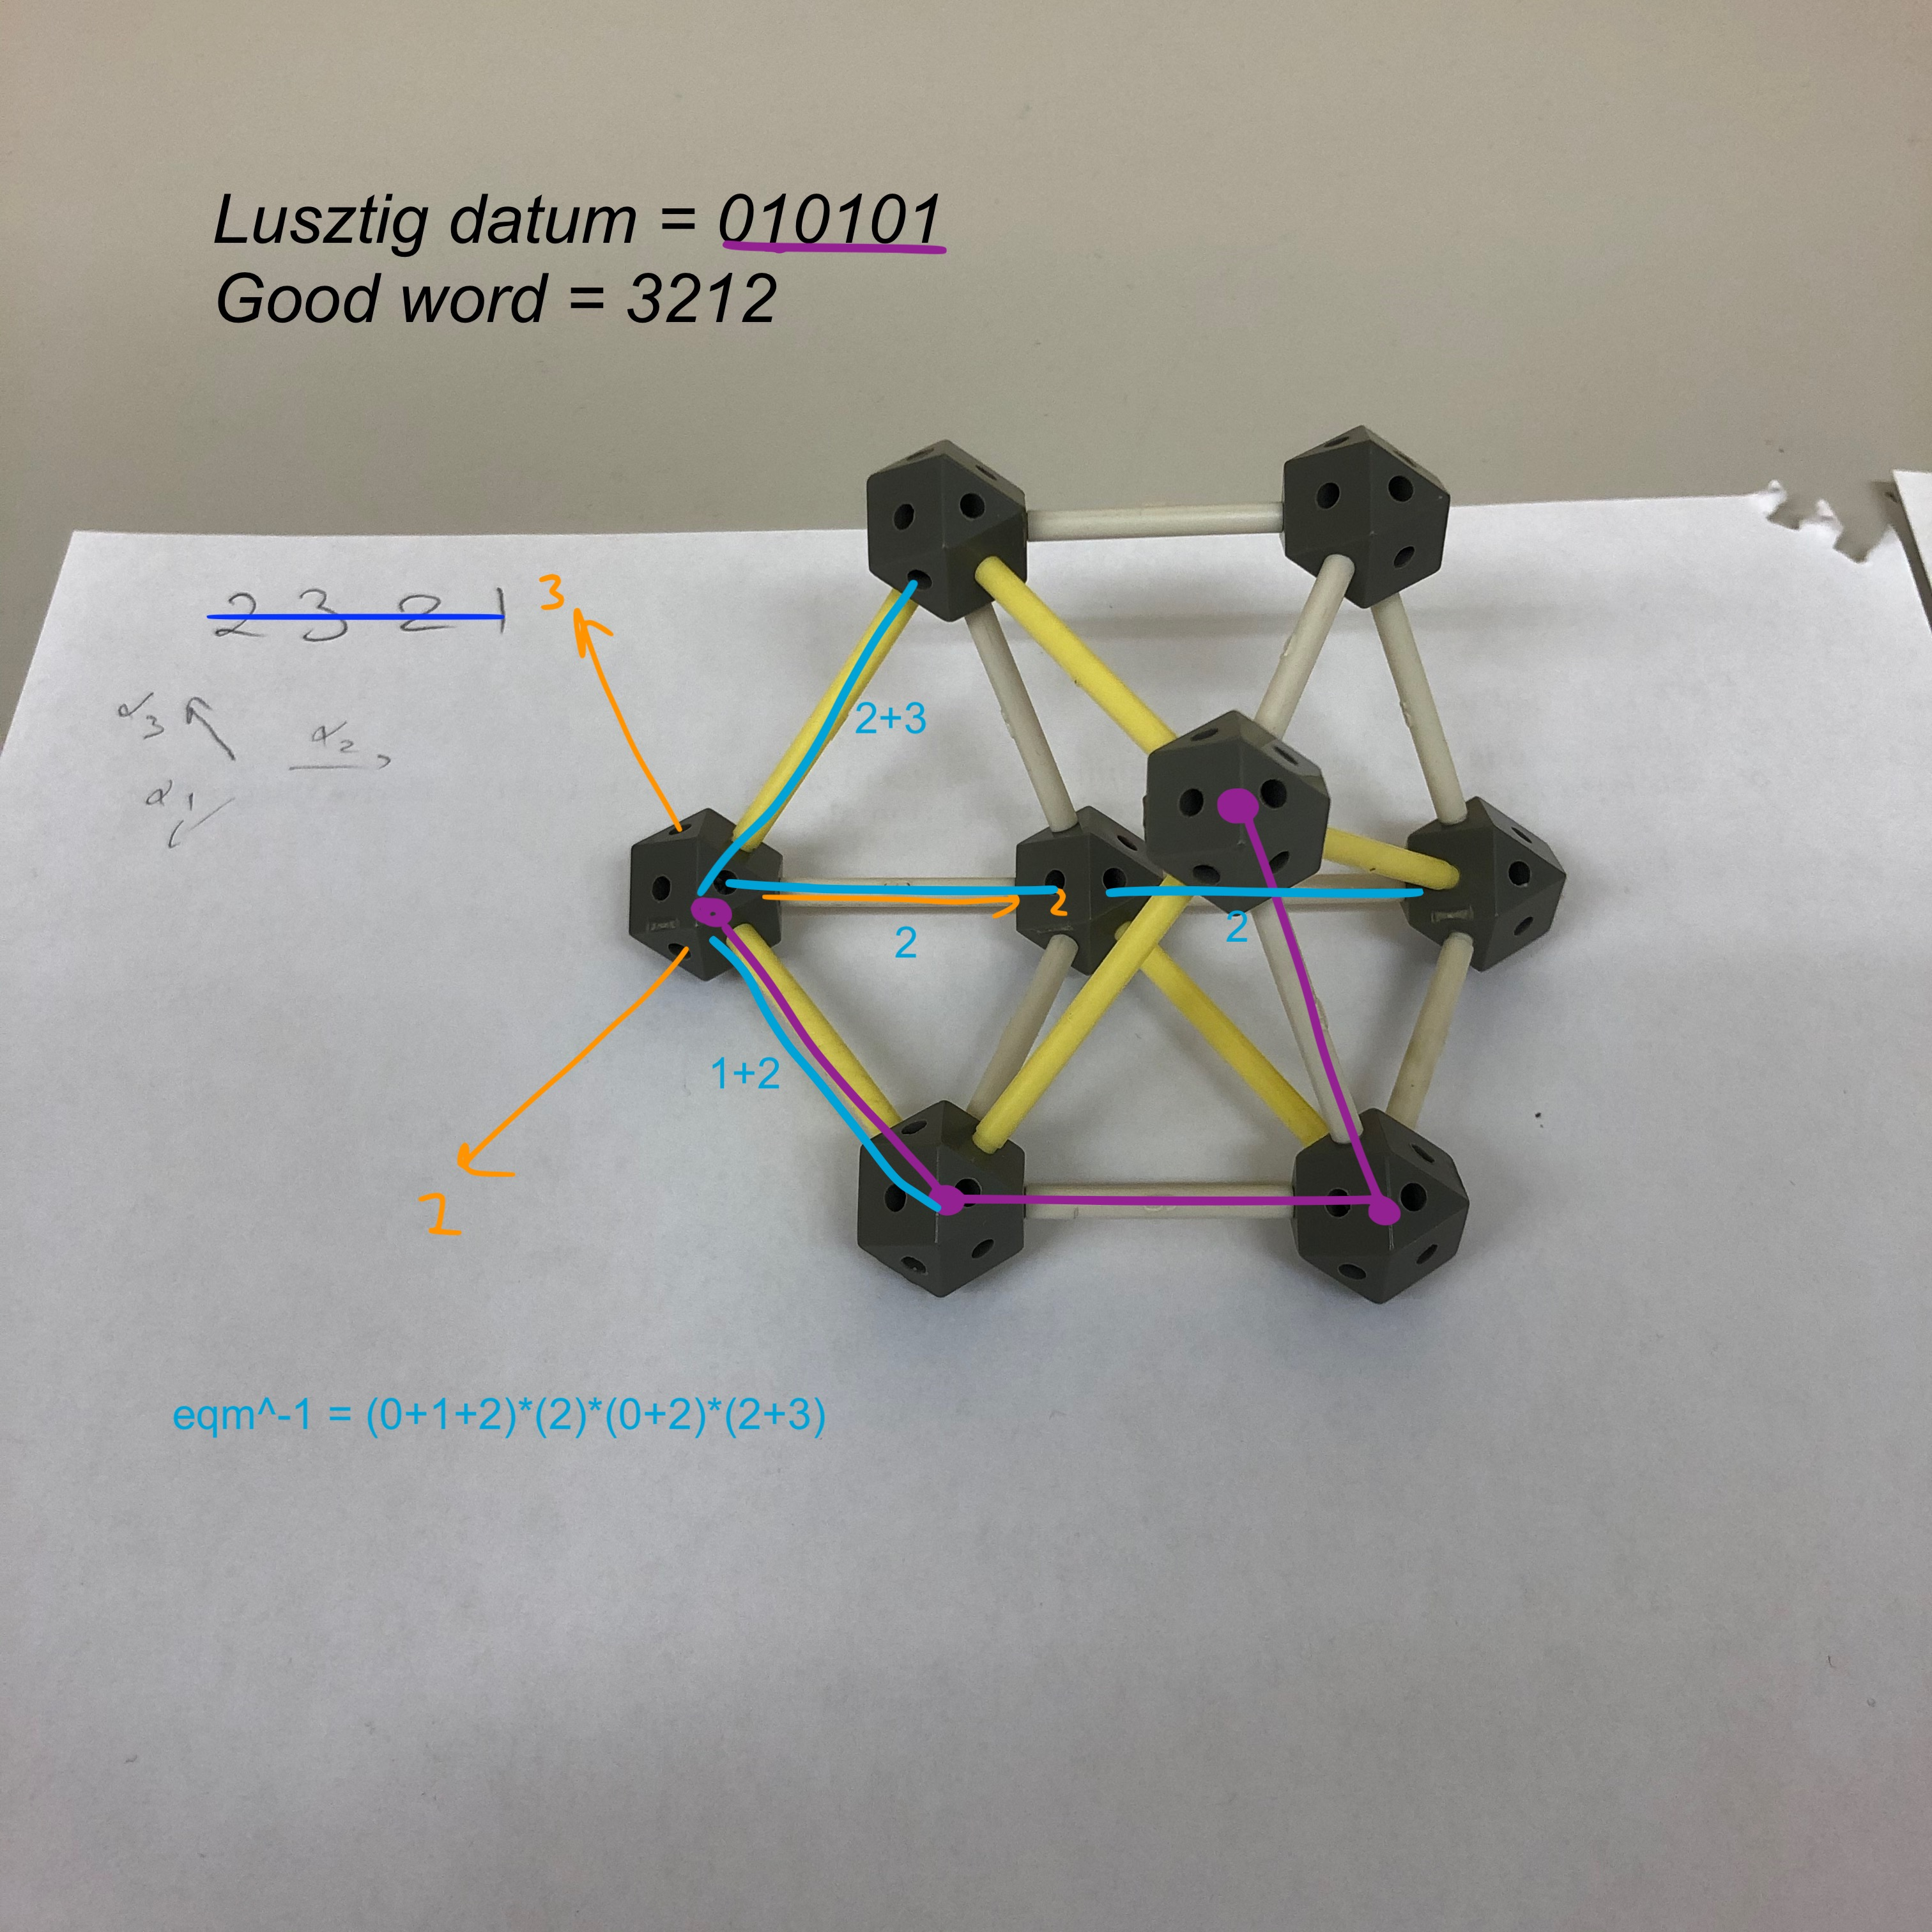
\includegraphics[height=100px]{img/3212.jpeg}
    % \end{center}
    % \caption{Lyndon word 3212}
    % \end{figure}

    From its tableau 
    $$
    \young(1113,223,4)
    $$
    we find the ideal of the corresponding MV cycle in
    {\small$$\begin{pmatrix}
        0&1&0&0&0&0&0&0\\
        0&0&1&0&0&0&0&0\\
        0&0&0&{a}_{1}&{a}_{2}&{a}_{3}&{a}_{4}&{a}_{5}\\
        0&0&0&0&1&0&0&0\\
        0&0&0&0&0&{a}_{6}&{a}_{7}&{a}_{8}\\
        0&0&0&0&0&0&1&0\\
        0&0&0&0&0&0&0&{a}_{9}\\
        0&0&0&0&0&0&0&0\end{pmatrix}
        \mapsto \begin{pmatrix}
            t^3 \\
            -a_1 -a_2t & t^2 \\
            -a_3 -a_4t & -a_6 - a_7 t & t^2 \\
            -a_5 & -a_8 & -a_9 & t 
        \end{pmatrix}
    $$}
    by imposing 
    $$
    \young(111,2)\subset\young(111,22)\subset\young(111,223)\subset\young(1113,223)
    $$
    so $I = \left({a}_{1},{a}_{2},{a}_{6},{a}_{3},{a}_{4}\right)$. We compute by hand 
    $$
    \mdeg I = (\alpha_1)(\alpha_1 + \hbar) (\alpha_1 + \alpha_2) (\alpha_1 + \alpha_2 + \alpha_3) (\alpha_2 )
    $$
    and so 
    $$
    \varepsilon^{T\times\CC^\times}_0(I) = \frac{1}{(\alpha_1 + \alpha_2 + \hbar)(\alpha_2 + \hbar) (\alpha_2 + \alpha_3) (\alpha_3 )}
    $$
    \item[{\bf 2.} $n_\bullet = (0,0,1,1,0,0)$:] $\lambda = (3,2,0,0)$ and $\mu = (2,1,1,1)$ \hfill 

    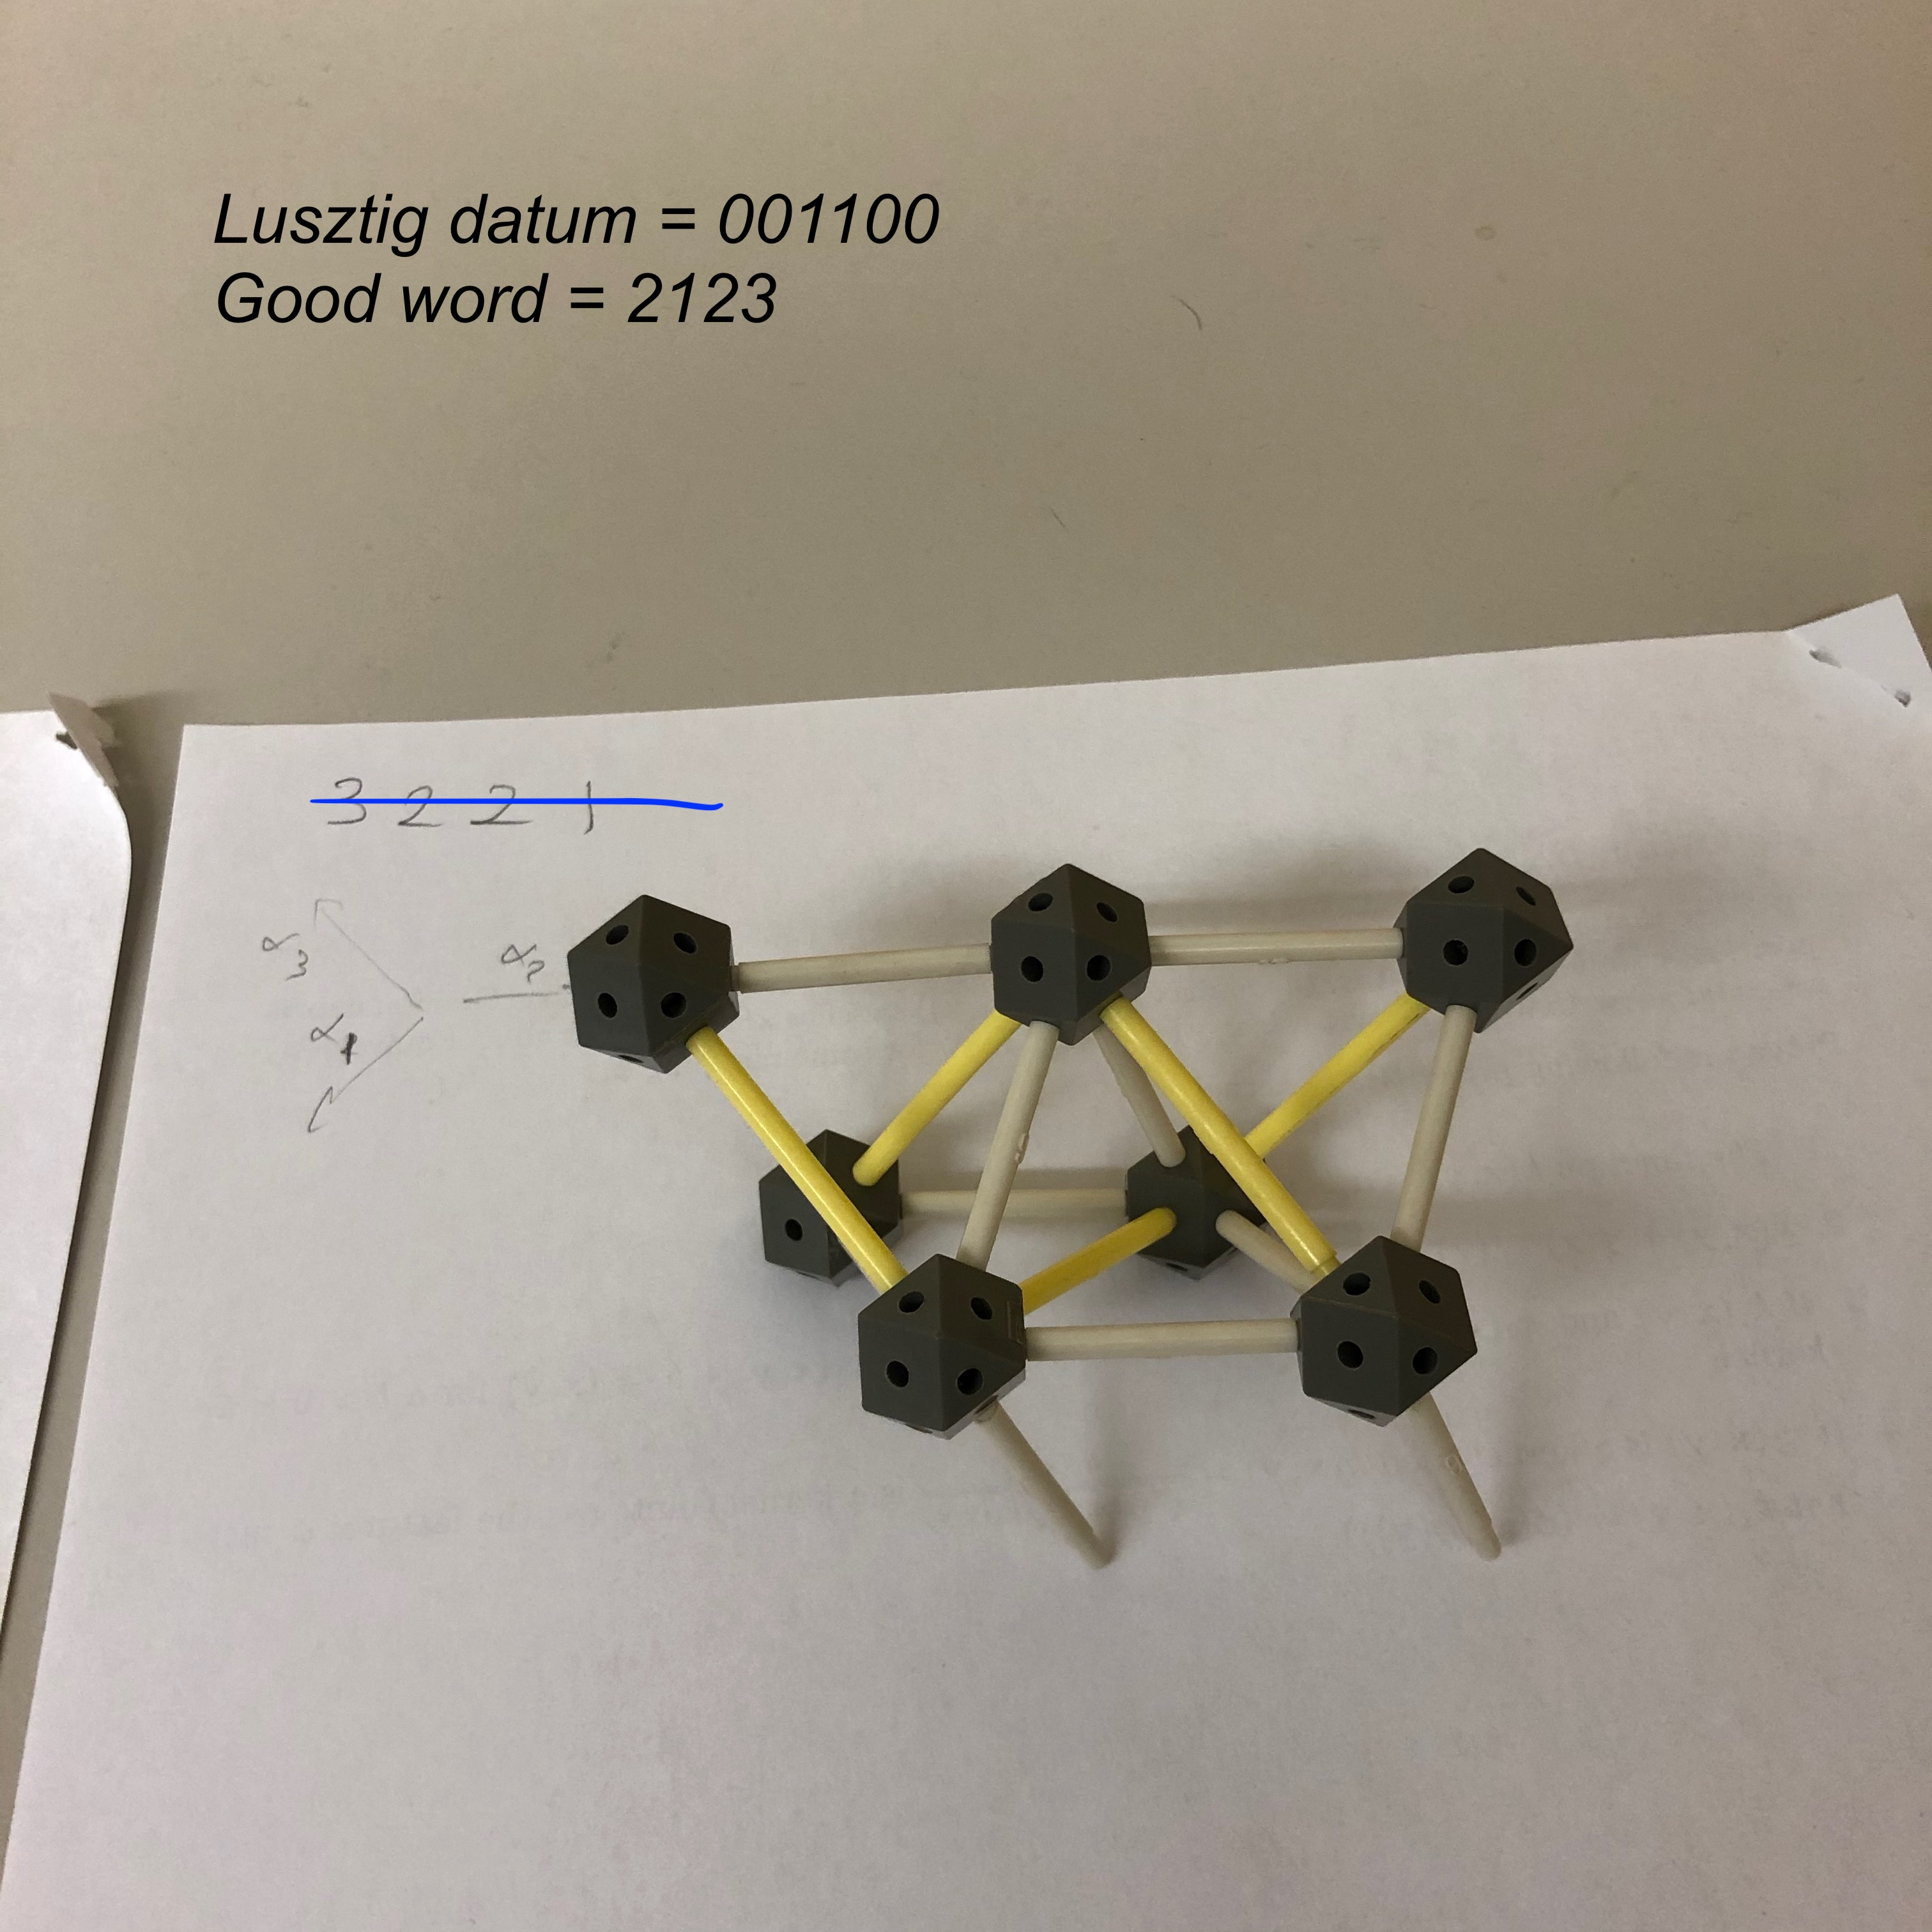
\includegraphics[height=100px]{img/2123.jpeg}

    From its tableau 
    $$
    \young(114,23)
    $$
    we find the ideal of the corresponding MV cycle in 
    $$\begin{pmatrix}
        0&1&0&0&0\\
        0&0&{a}_{1}&{a}_{2}&{a}_{3}\\
        0&0&0&{a}_{4}&{a}_{5}\\
        0&0&0&0&{a}_{6}\\
        0&0&0&0&0\end{pmatrix}\mapsto \begin{pmatrix}
            t^2 \\
            -a_1 & t \\
            -a_2 & -a_4 & t \\
            -a_3 & -a_5 & -a_6 & t 
        \end{pmatrix}$$
    by imposing 
    $$
    \young(11,2)\subset\young(11,23)
    $$
    so $I = (a_1,a_2)$. We compute by hand 
    $$
    \mdeg I = (\alpha_1) (\alpha_1 + \alpha_2)
    $$
    and so 
    $$
    \varepsilon^{T\times\CC^\times}_0(I) = \frac{1}{(\alpha_1 + \alpha_2 + \alpha_3)(\alpha_2)(\alpha_2 + \alpha_3)(\alpha_3)}
    $$
    \item[{\bf 3.} $n_\bullet = (0,1,0,0,1,0)$:] $\lambda = (2,2,0,0)$ and $\mu = (1,1,1,1)$ \hfill 

    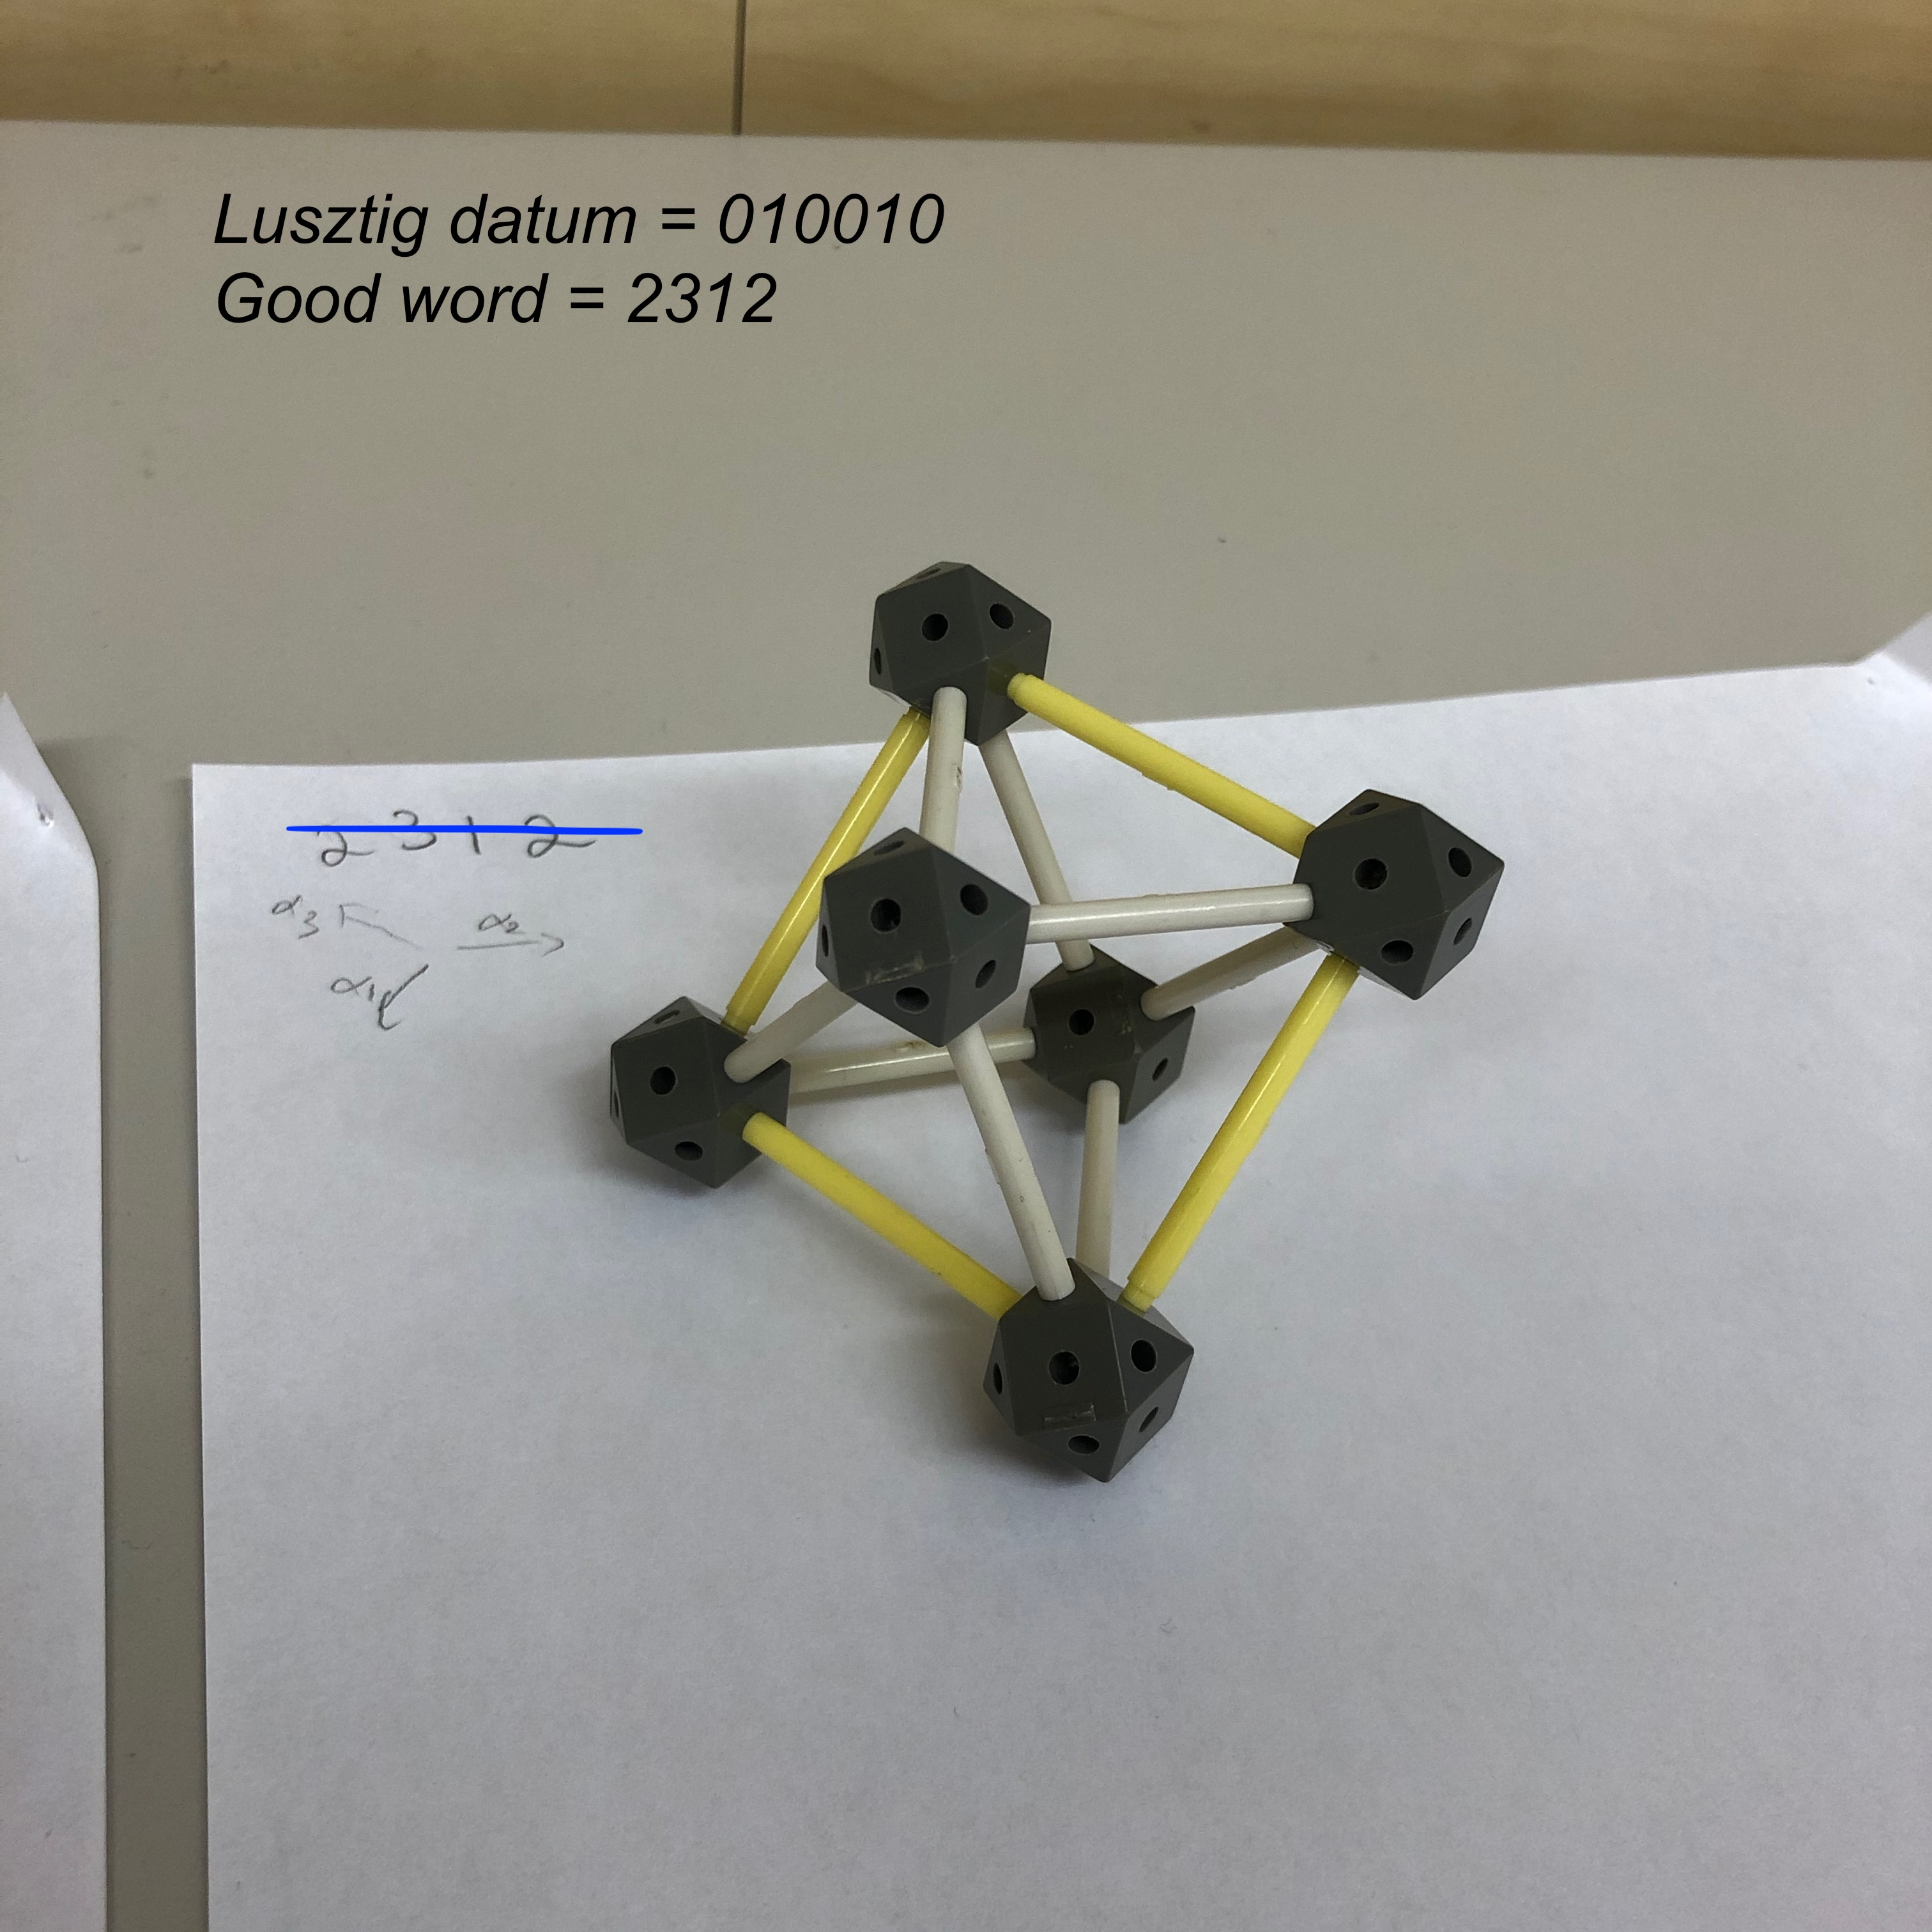
\includegraphics[height=100px]{img/2312.jpeg}

    From its tableau 
    $$
    \young(13,24)
    $$
    we find the ideal of the corresponding MV cycle in 
    $$\begin{pmatrix}
        0&{a}_{1}&{a}_{2}&{a}_{3}\\
        0&0&{a}_{4}&{a}_{5}\\
        0&0&0&{a}_{6}\\
        0&0&0&0\end{pmatrix}\mapsto \begin{pmatrix}
            t \\
            -a_1 & t \\
            -a_2 & -a_4 & t \\
            -a_3 & -a_5 & -a_6 & t
        \end{pmatrix}$$
    so $I = (a_1,a_6)$. We compute by hand 
    $$
    \mdeg I = (\alpha_1) (\alpha_3)
    $$
    and so 
    $$
    \varepsilon^{T\times\CC^\times}_0(I) = \frac{1}{(\alpha_1 + \alpha_2)(\alpha_1 + \alpha_2 + \alpha_3)(\alpha_2)(\alpha_2 + \alpha_3)}
    $$

    \item[{\bf 4.} $n_\bullet = (1,0,0,1,1,0)$:] $\lambda = (2,2,0,0)$ and $\mu = (1,1,1,1)$ \hfill 

    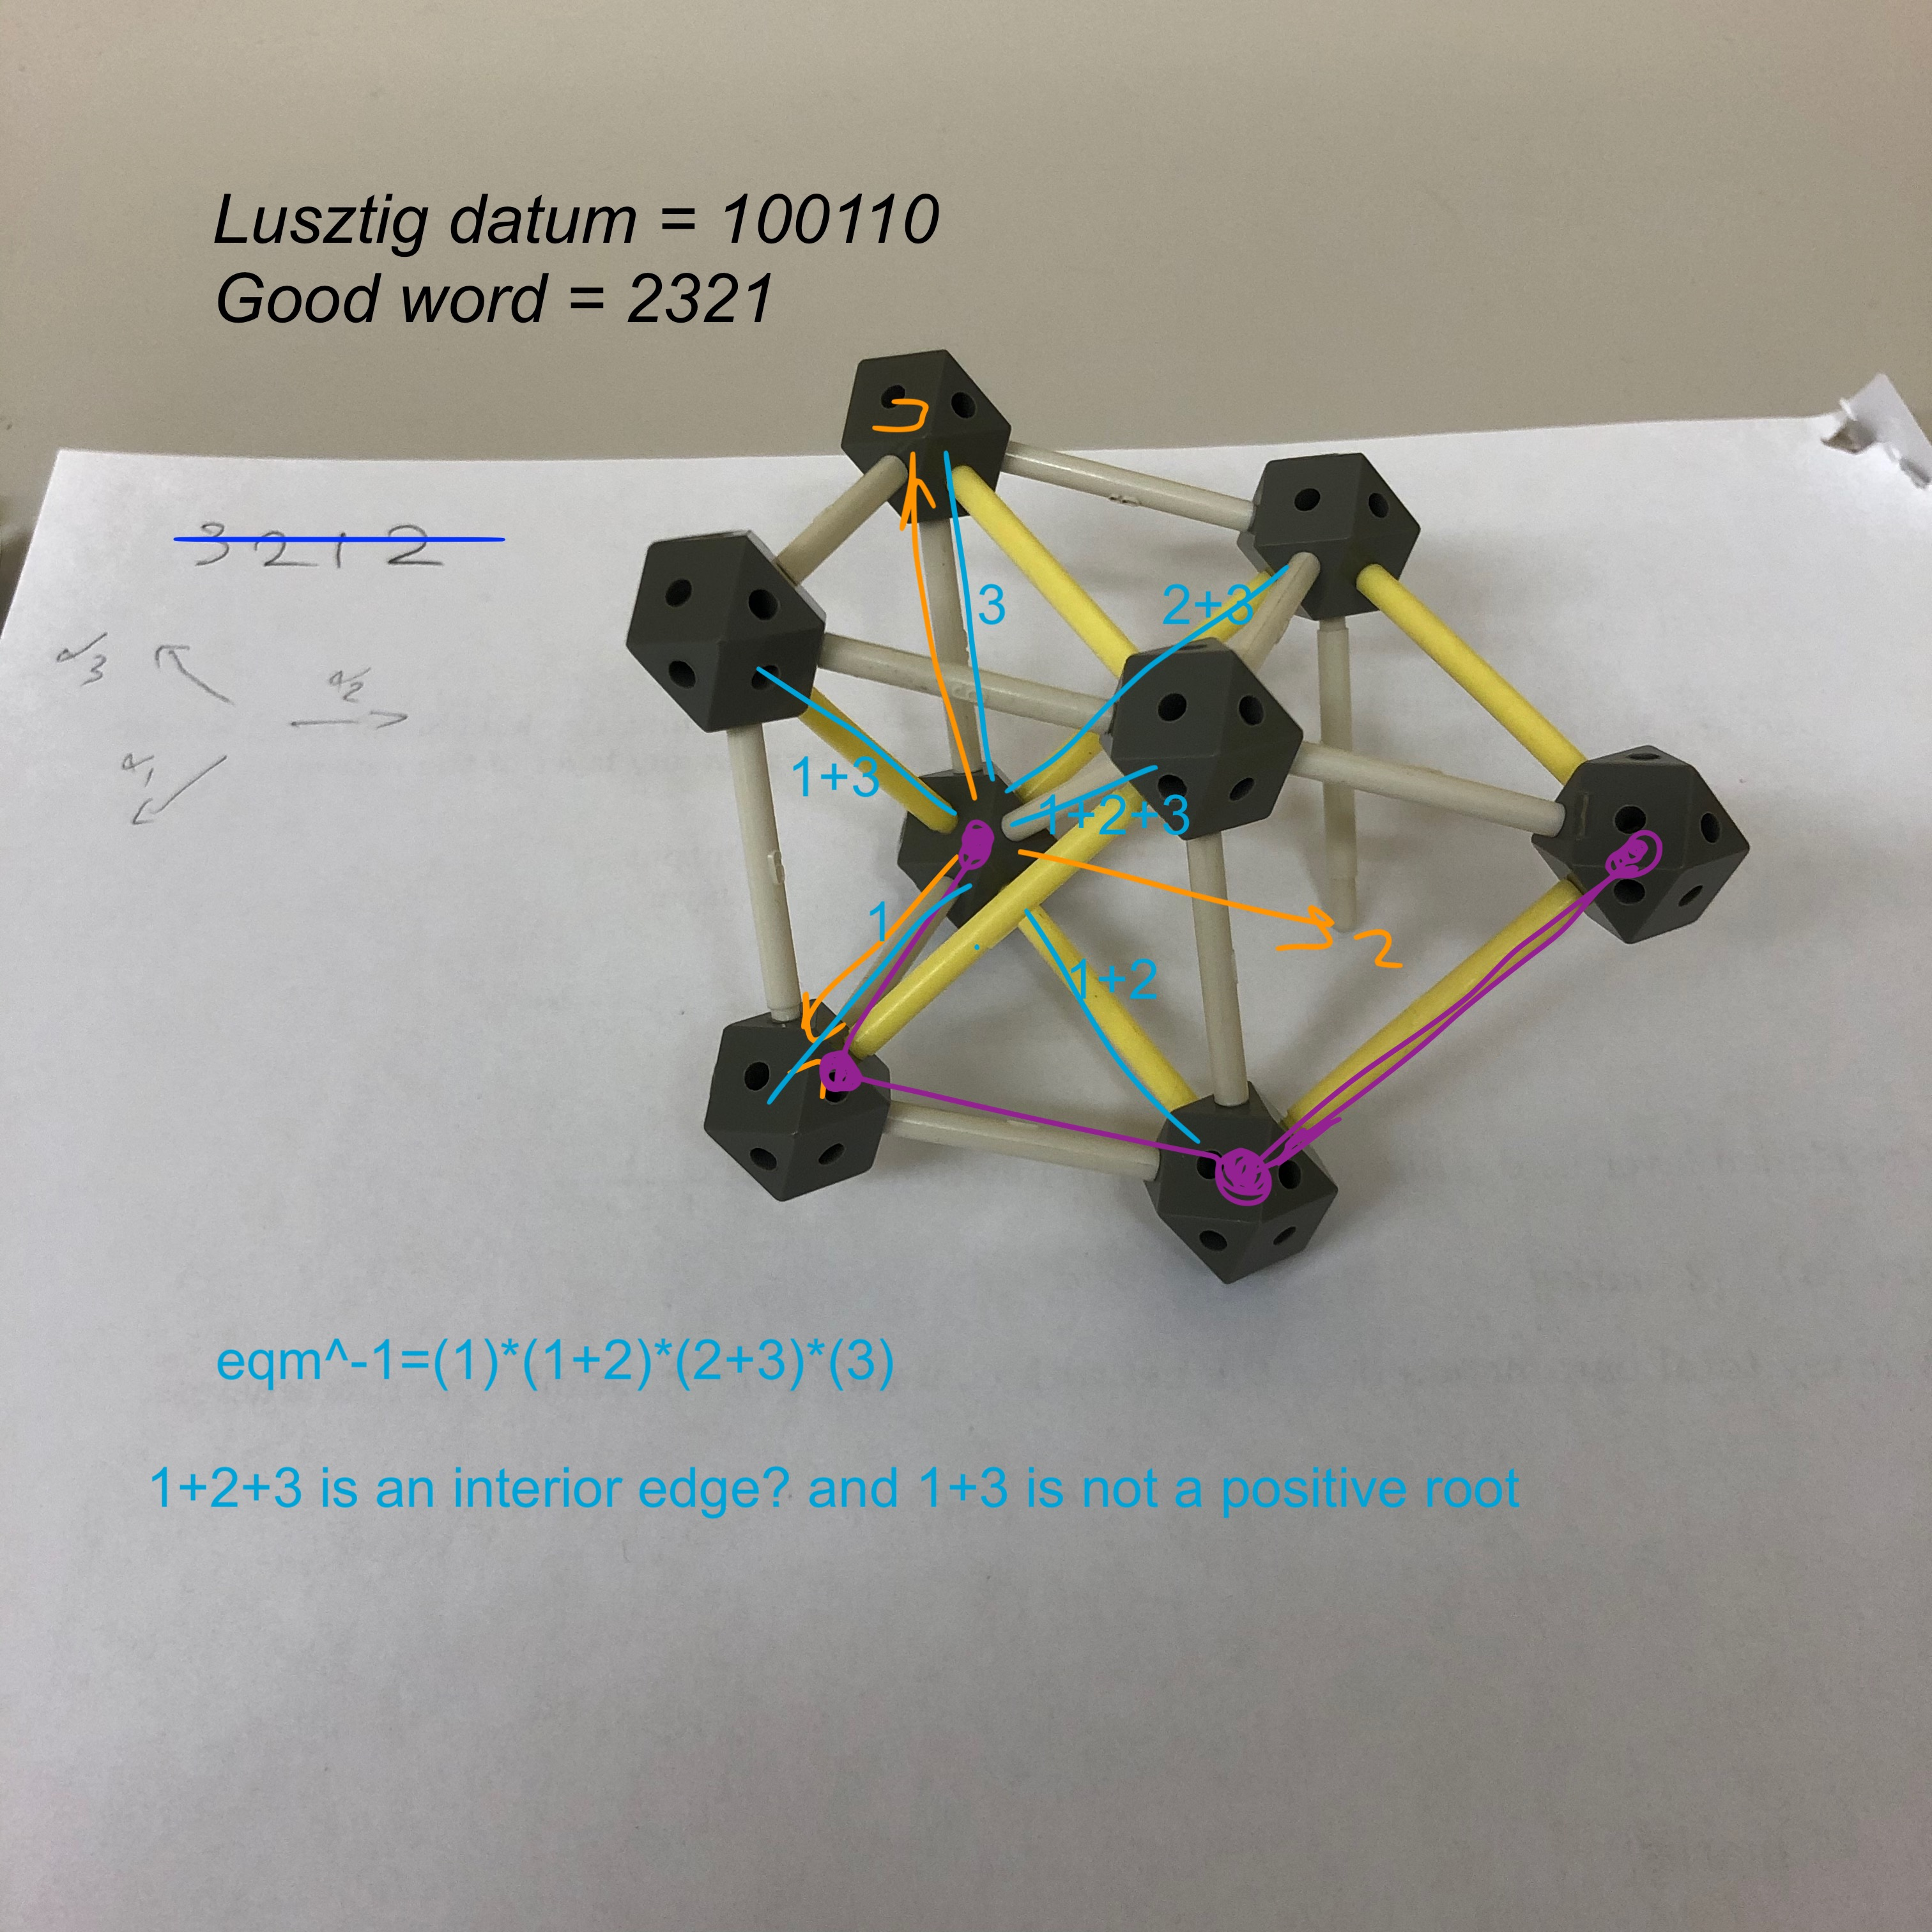
\includegraphics[height=100px]{img/2321.jpeg}

    From its tableau 
    $$\young(12,34)$$
    we find the ideal of the corresponding MV cycle in 
    $$\begin{pmatrix}
        0&{a}_{1}&{a}_{2}&{a}_{3}\\
        0&0&{a}_{4}&{a}_{5}\\
        0&0&0&{a}_{6}\\
        0&0&0&0\end{pmatrix}\mapsto \begin{pmatrix}
            t \\
            -a_1 & t \\
            -a_2 & -a_4 & t \\
            -a_3 & -a_5 & -a_6 & t
        \end{pmatrix}$$
    so $I = \left({a}_{4},{a}_{1}{a}_{5}+{a}_{2}{a}_{6}\right)$. 
    We compute by hand 
    $$
    \mdeg I = (\alpha_2) (\alpha_1 + \alpha_2 + \alpha_3)
    $$
    and so 
    $$
    \varepsilon^{T\times\CC^\times}_0(I) = \frac{1}{(\alpha_1)(\alpha_1 + \alpha_2)(\alpha_2 + \alpha_3)(\alpha_3)}
    $$
    \item[{\bf 5.} $n_\bullet = (1,0,0,2,0,1)$:] $\lambda = (3,3,1,0)$ and $\mu = (2,2,2,1)$ \hfill 

    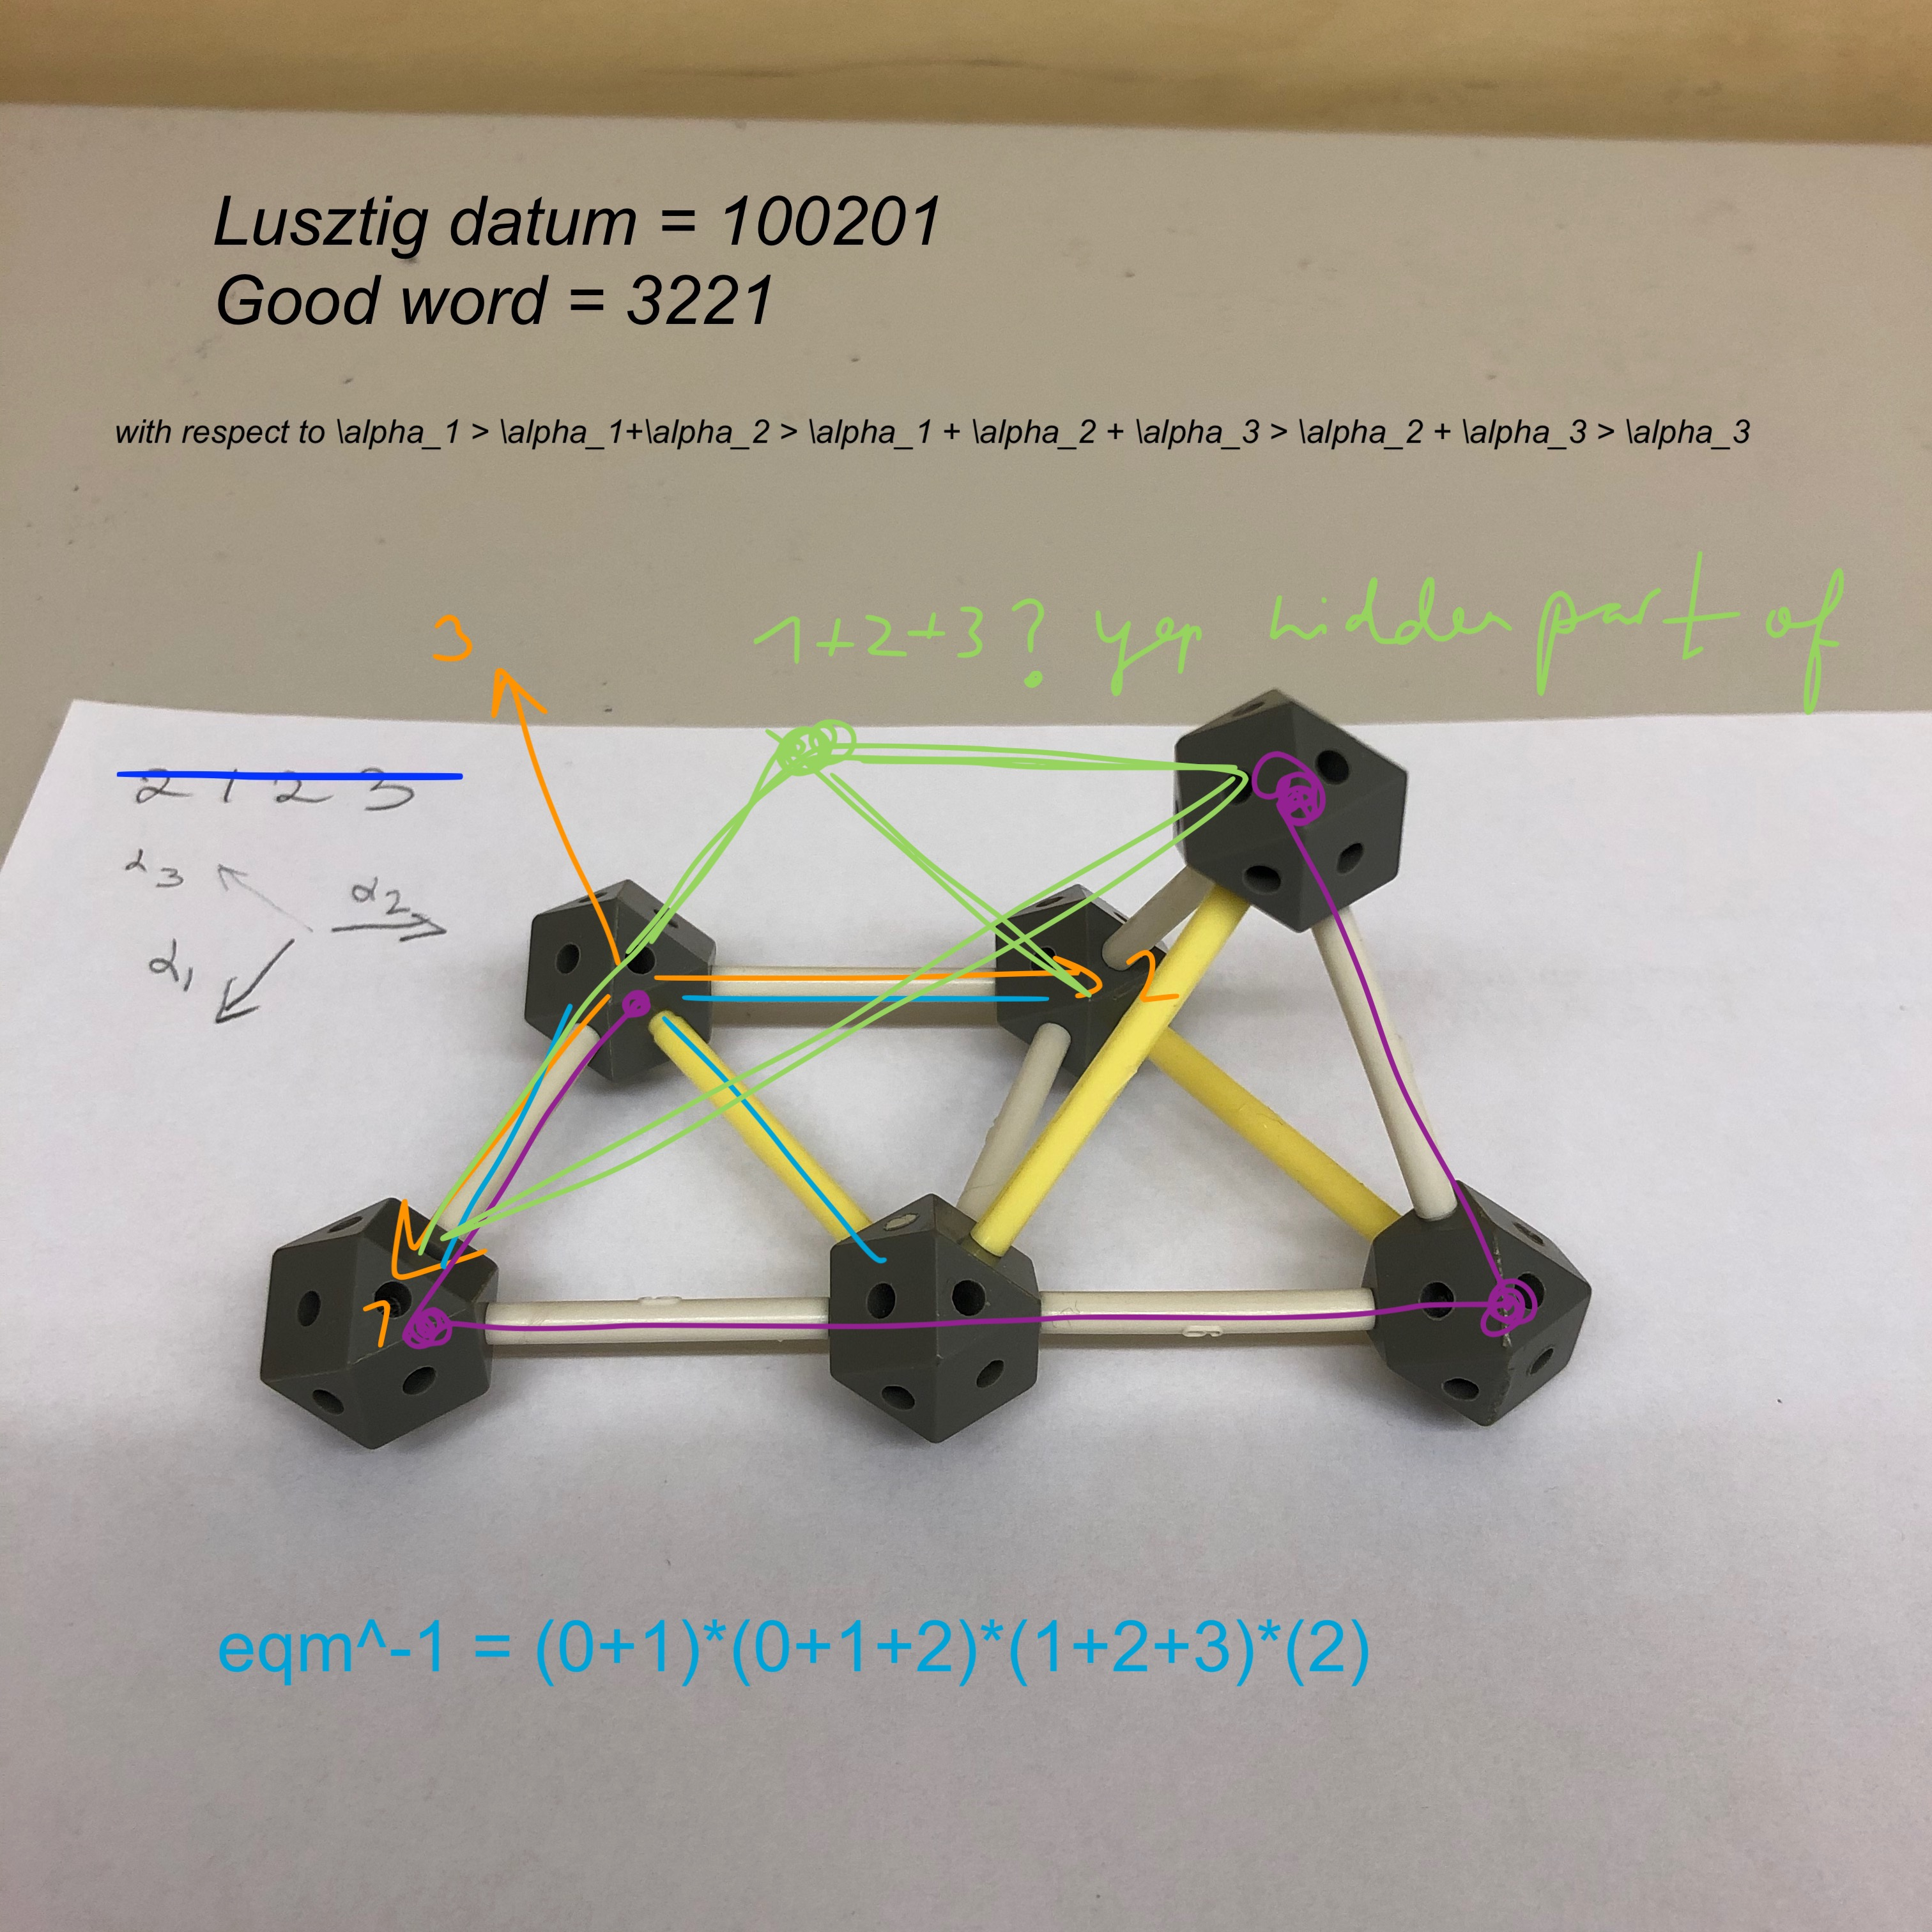
\includegraphics[height=100px]{img/3221.jpeg}

    From its tableau 
    $$\young(112,233,4)$$
    we find the ideal of the corresponding MV cycle in 
    $$\begin{pmatrix}
        0&1&0&0&0&0&0\\
        0&0&{a}_{1}&{a}_{2}&{a}_{3}&{a}_{4}&{a}_{5}\\
        0&0&0&1&0&0&0\\
        0&0&0&0&{a}_{6}&{a}_{7}&{a}_{8}\\
        0&0&0&0&0&1&0\\
        0&0&0&0&0&0&{a}_{9}\\
        0&0&0&0&0&0&0\end{pmatrix} \mapsto \begin{pmatrix}
            t^2 & \\
            - a_1 - a_2 t & t^2 \\
            -a_3 -a_4 t & -a_6 - a_7t & t^2 \\
            - a_5 & -a_8 & -a_9 & t
        \end{pmatrix}
    $$
    by imposing 
    $$
    \young(11,2) \subset \young(112,2) \subset \young(112,23) \subset \young(112,233)
    $$
    so $I = \left({a}_{2},{a}_{6},{a}_{1},{a}_{9},{a}_{3}\right)$. 
    We compute by hand 
    $$
    \mdeg I = \alpha_1(\alpha_1 + \hbar)(\alpha_1 + \alpha_2)(\alpha_2)(\alpha_3)
    $$ and so 
    $$
    \varepsilon^{T\times\CC^\times}_0(I) = \frac{1}{(\alpha_1 + \alpha_2 + \hbar)(\alpha_1 + \alpha_2 + \alpha_3)(\alpha_2 + \hbar)(\alpha_2 + \alpha_3)}
    $$
\end{description}

%
% import bibliography from tex.bib file
%
\bibliographystyle{plain}
\bibliography{tex}
%
% for bundling, bbl file contains
%
% \begin{thebibliography}{E-G-S}

% \bibitem[A1]{Anderson00}
% J.~E.~Anderson, \textit{On Mirkovi\'c and Vilonen's Intersection Homology cycles for the Loop Grassmannian.} PhD thesis, Princeton University, 2000.

% \end{thebibliography}
%
\end{document}